\section{Literaturvergleich der gemessenen Werte} \label{Messlit}

Im folgenden werden die Literaturwerte \cite[S. 1474]{CRCHandbook2003} mit den gemessenen Werten verglichen. Dabei wird der Peak im Diagramm abgelesen und dann der dazugehörenden 
exakt Messwert der x-Achse in den Daten nachgeschlagen. Die nicht in der Literatur erwähnten Peaks werden außenvor gelassen, da sie vermutlich zu dem in der Lampe verwendetem Edelgas 
gehören. Daraufhin wird die Differenz des Literaturwertes mit dem des Messwerts berechnet und der Messfehler des jeweiligen Messwertes ermittelt. Diese wird dann in der Grafik \ref{FehlUeb} 
in einem Diagramm aufgetragen.
\begin{table}[h]
    \centering
    \begin{tabular}[h]{l|c|c|r}


        Literaturwerte in \r{A} & Messwerte in \r{A} & Betrag der Differenz in \r{A} & Fehler der Messung in \r{A}\\
       \hline
       %Nicht in der Literatur  & 3135 & sdfgsdf \\
       3650.15  & 3655 & 4.85 & 3.7\\
       4046.56  & 4045 & 1.56 & 3.7\\
       4358.34 & 4360 & 1.66  & 3.7\\
       5460.75 & 5460 & 0.75 & 3.7\\
       5769.6  & 5770 & 0.4 & 3.7\\
       5790.7  & 5795 & 4.3 & 3.7\\
       6234.4  & 6265 & 30.6 & 3.7\\
       7346  & 7305 & 41.0 & 3.7\\
       %Nicht in der Literatur  & 8100 & asdf \\
       %Nicht in der Literatur  & 8730 & asdf \\
\end{tabular}
    \caption{Vergleich der gemessenen Werte mit den Literaturwerten}
\end{table}
Verwede zur Berechnung der Fehler folgende Formel:
\begin{equation}
    \Delta \lambda = \sqrt{2} \cdot\frac{b}{f}*s_e 
\end{equation}
Hierbei ist $b$ die Gitterkonstante, $f$ die Hohlspiegelbrennweite und $s_e$ die Breite des Ein-/Austrittsspaltes.\\
\newline
\begin{tabular}[h]{l r}
    Gitterkonstante $b$ & $833 nm$\\
    Hohlspiegelbrennweite $f$ & $250mm$\\
\end{tabular}
\\
\newline
Wenn man dies in einem Diagramm aufträgt, sieht man sehr schön, dass Differenz und Messfehler in der gleichen Größenordnung liegen. Dabei werden nur die Hauptemmissionslinien 
aufgetragen, da diese sehr eindeutig zuordenbar sind. Die aufgetragenen Linien sind die Linien bei 365nm, 404nm, 435nm, 576,9nm und 579,07nm.
\begin{figure}[h]
    \centering
    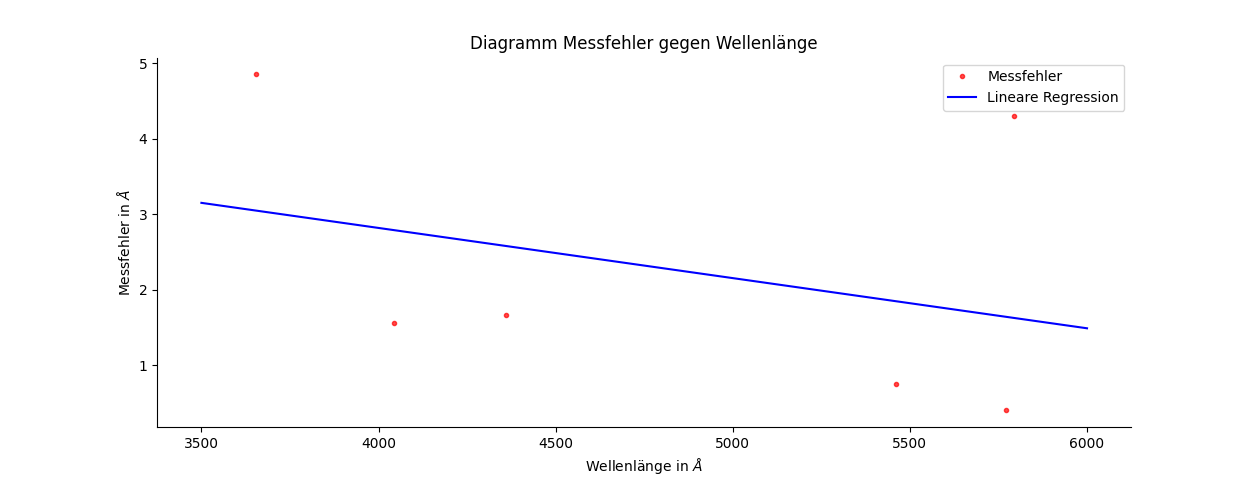
\includegraphics[width =\linewidth]{linregress.png}
    \caption{Fehler in der Übersichtsmessung}
    \label{FehlUeb}
\end{figure}